\documentclass{emulateapj}
\usepackage{natbib}
%\usepackage{color}
%\usepackage{xspace}
\citestyle{aa}

\shorttitle{} 
\shortauthors{Leonidas Moustakas et al.}

\begin{document}
\bibliographystyle{apj}

\submitted{}

%\def\ltsima{$\; \buildrel < \over \sim \;$}
%\def\lsim{\lower.5ex\hbox{\ltsima}}
%\def\gtsima{$\; \buildrel > \over \sim \;$}
%\def\gsim{\lower.5ex\hbox{\gtsima}}

\title{CLASH: Galaxy Formation Constraints from Distant Spatially Extended Strongly Lensed Galaxies} 

\author{Leonidas A. Moustakas\altaffilmark{1}}
\author{Genevieve Graves\altaffilmark{2}}
\author{John Moustakas\altaffilmark{3}}
\author{CLASH Team\altaffilmark{4}}
\altaffiltext{1}{JPL/Caltech}
\altaffiltext{2}{UC Berkeley}
\altaffiltext{3}{UCSD}
\altaffiltext{4}{Planet Earth}

\begin{abstract}
Opening statement on fundamental questions of galaxy formation, and
the bifurcation of a couple basic scenarios.  These scenarios lead to
predictions, including fairly nuanced or sophisticated measurements
that one can make of individual galaxies, such as metallicity tracers
and the like.  For very distant or intrinsically faint galaxies these
are very difficult observations to make, and are more suited for the
GSMT or JWST eras. An opening foray can be made through a detailed
exploration of internal variations of the stellar populations. While
impractical when galaxies at high redshift are only modestly resolved
by \emph{HST}, we can take advantage of the significant 10-100x
stretching and reprojection of galaxies that are lensed by foreground
massive galaxy clusters. We report on a pilot analysis of twenty such
objects, between redshifts $z\sim1-3$, lensed by clusters targeted by
the CLASH survey, and therefore with 16 \emph{HST} bands of $\sim1$
orbit depth each and spanning NUV through the NIR.  Because the
lensing process is fully stochastic, this is essentially a
fortuitously discovered and random sample of distant lensed
galaxies. We do sophisticated stellar population synthesis analysis
across many resolution elements of each galaxy, and derive the
spatial variance in key model parameters. We find some cool stuff. 
\end{abstract}
\keywords{gravitational lensing}

\section{Introduction} 

% (\citealt{bunker:00})

The goal of this project is to characterize the stellar populations of
high-redshift lensed galaxies and contrast them with a lower-redshift
comparison sample.  By separately fitting the SEDs of spatially
resolved galaxy segments, we aim to characterize the distribution of
star formation in high-z galaxies, identify passively evolving stellar
components, and if possible compare the metallicities of the various
components to identify the source of the star-forming gas.  In a
separate but similar project, we will use lensed, edge-on star-forming
galaxies with clear dust lanes to characterize the dust absorption
spectrum in these galaxies.  For both projects, we will make use of
the full set of 16-band HST photometry that is being acquired by the
CLASH collaboration.

The tasks described in \S\ref{targets}-\ref{apertures} are necessary
for both projects.  The SED-fitting project with further require
running the ISEDFIT model of J. Moustakas in order to obtain stellar
population information.  In contrast, the dust-SED fitting will be an
empirical comparison of the dust-obscured and non-dust-obscured
regions of individual galaxies, and therefore does not require the use
of ISEDFIT.  I (G. Graves) therefore propose that the SED-fitting
project be led by L. \& J. Moustakas, while the dust-SED project be
led by myself, but this is of course open to discussion and may evolve
as the project progresses.

\subsection{Gradients in Spiral Galaxies}

{\bf Metallicity gradients:} I think it is pretty well established that
spiral galaxies have substantial metallicity gradients, with
metal-rich centers and metal-poor outer parts.  People have done this
looking at stellar metallicity gradients with colors in other galaxies
\citep[e.g.][]{Bell:00}, with stellar spectra in our own galaxy
\citep[e.g.][]{Ivezic:08}, and by mapping the metallicity gradients
of HII regions in star-forming galaxies \citep[e.g.][]{Zaritsky:94}. 
  
{\bf Age gradients:} There are multiple studies that suggest that spirals
also have significant age gradients, with older stars in the center
and younger stars in the outer parts.  e.g., Bell \& de Jong (2000)
fit SEDs to radially resolved optical and near-IR photometry and find
the centers of galaxies to be old and metal-rich, while the outer
parts are younger and more metal-poor.  Kauffmann et al. (2006) find
that many massive bulge-dominated galaxies have blue outer regions,
which appear to show residual star formation even after star formation
has ceased in the inner part of the galaxy.

\subsection{Gradients in Early Type Galaxies}

\citep{Somerville:2003aa}, \citep{Ferguson:2004qw},
\citep{Moustakas:1998tn}. 

{\bf Metallicity gradients:} It is well-established that early type galaxies
show strong metallicity gradients, with metal-rich centers and
metal-poor outer parts.  The SAURON team (Scott, Cappellari et
al. 2009) recently published this in an interesting and somewhat novel
way---plotting [Z/H] as a function of the local escape velocity in the
galaxy (essentially a radial gradient, with high Vesc in the center).
There are many other studies that show similar things, both with
spectral absorption line strengths and colors.

{\bf Age gradients:} These are more debated.  The Scott et al. (2009) paper
mentioned above find age gradients that are flat in some galaxies,
while other show youngish central ages and older ages farther out.
Another relevant paper is Sanchez-Blazquez et al. (2007), who find
weak or no age gradient in 10/11 early types, while one have a very
young center.  Interestingly, the weak positive age gradients,
combined with the negative metallicity gradients, means that the
age-metallicity degeneracy acts to keep galaxy color (and
line-strength) gradients weaker than they otherwise might be.

{\bf Abundance ratio gradients:} There do not seem to be strong [alpha/Fe]
gradients in early types.  In the papers quoted above, Scott et
al. (2009) find no [alpha/Fe] gradients and Sanchez-Blazquez et
al. (2007) find no gradients, weak positive gradients, or weak
negative gradients in their galaxies.

Gradients beyond the half-light radius: In general, these studies do
not go beyond the half-light radius of the galaxy.  Some work that I
am doing right now tracing stellar population gradients out to 2-3
Reff essentially agrees with these studies: Age gradients vary from
galaxy-to-galaxy, are usually weak, but with some galaxies showing
young cores.  All galaxies show strong negative gradients in total
metallicity.  [alpha/Fe] varies little with radius.  Interestingly,
carbon-enhancement ([C/Fe]) seems to scale strongly with
radius---galaxies have much higher [C/Fe] in their centers that in
their outskirts.

{\bf At high redshift -- stuff happens. }

It is of course much harder to study population gradients at high
redshift.  Rigby et al. (2011) and Wuyts et al. (2010) have SEDs and
spectroscopy for a lensed galaxy at z=1.7, but don't try to extract
spatially-resolved information.  There was a Rigby HST proposal in
Cycle 18 to do resolved SED fitting for a lensed arc (might well be
the same one) which I think got time, but I don't see the paper out
yet.

{\bf Theory}

Spiral galaxies: I don't know much about formation models for spiral
galaxies.  Bell \& de Jong (2000) propose a scenario in which star
formation happens early and rapidly in high-density regions of the
galaxy (i.e., the center) and proceeds more slowly out at large radius
where the gas densities are low, hence leaving low-lever star
formation in the outer parts of the galaxy at late times.  There is a
huge literature on the Milky Way star formation history and detailed
chemical evolution models with which I am not very familiar.  Some
names that spring to mind are Brad Gibson, Rok Roskar, Daisuke Kawata,
Chiaki Kobayashi.  I'm sure I'm missing some big ones.

Early-type galaxies: There are limited numbers of chemical evolution
models for early type galaxies (Gibson et al. 2007, Pipino et
al. 2010), and they tend to be trying to reproduce existing
observations, not making strong new predictions.  An interesting
recent paper is Oser et al. (2010).  They model massive early type
galaxies using a hydro-code super-posed on a zoom-in of a cosmological
N-body simulation.  Their galaxies wind up containing two
sub-populations of stars, those that formed "in situ" in the massive
halo, and those that formed in satellites outside Rvir of the main
halo, which were then accreted at later times.  The in situ stars
dominate the central part of the galaxy, while the accreted stars wind
up at much higher radius, thus setting up a strong gradient in the
origin of the stars.  Interestingly, both the in situ stars and the
accreted stars tend to be old.  There is often a little dribble of
residual in situ star formation in their models of less massive
galaxies, which would tend to make the central population younger.
Also, you'd expect strong differences in the metallicities of the two
components, with the in situ stars showing much higher metallicities
than those that were accreted from small satellites, due to the
mass-metallicity relation and the greatly reduced ability of small
galaxies to hold onto metal-enriched SN ejecta.


The power of strong gravitational lensing as a tool towards a broad
range of astrophysical discoveries. (Reference to some lensing school
notes, eg the Saas Fee lectures). The lensing object (REF), magnified
background sources (\citealt{bunker:00}), and indeed for cosmology
(Coe \& Moustakas, submitted). Lots of references here for background,
nothing too profound.

To these ends, since the first strong lens was discovered by
\citet{walsh:79}, both serendipity and systematic programs have
uncovered several hundred strong lenses by the present day. Broadly
speaking, these have been found through one of two techniques, whether
serendipitous or through a structured and pre-determined strategy. The
first exploits the remarkable visual geometry of lenses in space- or
ground-based imaging data (e.g. MDS \citet{ratnatunga:99}, EGS
\citet{moustakas:07}, SL2S \citet{cabanac:07}, HAGGLeS
\citet{marshall:09}). The second is spectroscopic, and relies on the
observation of ``anomalous'' spectroscopic features.

This latter approach was pioneered by \citet{warren:96}, and has come
to spectacular fruition by the Sloan Lens ACS (SLACS) Survey
\citep{bolton:08}, which has confirmed some one hundred new strong
galaxy-galaxy lenses by \emph{Hubble} imaging follow-up to
spectroscopically identified candidates.  While the efficiency
afforded by the Sloan spectroscopic database is high, lenses have been
uncovered through regular ground-based spectroscopic observations
(e.g.~\citealt{bolton:06}).  In this paper we report on similarly
discovered lenses, in several distant galaxy clusters, which all
happen to be from the X-ray flux-limited Massive Cluster Survey (MACS)
sample of \citet{ebeling:01}. 

The observations are described in the following section, followed by a
more detailed presentation of the lenses and the available data.  We
end with a discussion of the lensing rates implied by these
discoveries, how other surveys may fare, and the general utility of
such lenses. All magnitudes are given in AB, and where relevant we
adopt a concordance cosmology. 

% 
 \begin{center}
 \begin{table*}[t]
 \begin{center}
 \scriptsize
 \caption{\label{tab:data}}
 \begin{tabular}{cccccccc}
 \hline\hline
 \multicolumn{1}{c}{RA} & 
 \multicolumn{1}{c}{Dec} & 
 \multicolumn{1}{c}{Cluster} & 
 \multicolumn{1}{c}{$m_{\rm filter}$} &
 \multicolumn{1}{c}{$\theta_{\rm E}$} & 
 \multicolumn{1}{c}{$z_{\rm lens}$} & 
 \multicolumn{1}{c}{$z_{\rm source}$}&
 \multicolumn{1}{c}{Notes}\\
 %%
 \multicolumn{2}{c}{J2000} & 
 \multicolumn{1}{c}{} & 
 \multicolumn{1}{c}{AB} & 
 \multicolumn{1}{c}{arcsec} & 
 \multicolumn{1}{c}{} & 
 \multicolumn{1}{c}{} & 
 \multicolumn{1}{c}{}\\
 \hline
 00:25:23.487 & $-$12:19:42.8 & MACS\,J0025.4$-$1222  & $30.0$                  & $1.0\pm0.3$ & 0.582 & 2.047 & \\
 17:20:06.416 & $+$35:35:26.3 & MACS\,J1720.3$+$3536 & $r_{\rm SDSS}=20.6$ & $1.0\pm0.3$ & 0.384 & 2.132 & \\
 17:20:18.486 & $+$35:37:12.8 & MACS\,J1720.3$+$3536 & $r_{\rm SDSS}=19.1$ & $1.0\pm0.3$ & 0.385 & 2.787 & \\
 21:29:19.973 & $-$07:42:18.2 & MACS\,J2129.4$-$0741 & $r_{\rm SDSS}=21.6$  & $1.0\pm0.3$ & 0.594 & 1.211 & AGN Source\\
 \end{tabular}
 \end{center}
 \end{table*}
 \end{center}


% 
% 
% \section{Observations}

%%%%%%%%%%%%%%%%%%%%%%%% Target Selection!! %%%%%%%%%%%%%%%%%%%

\section{Target Selection}\label{targets}

We need to identify lensed sources that are bright enough and extended
enough for resolved SED analysis.  Targets should also have
spectroscopic redshifts.  Two types of targets are particularly of
interest: those with obvious clumpy structures that are ideal for
resolved SED fitting, and those that appear to be lensed edge-on
star-forming galaxies with strong dust lanes.

Genevieve has made a first pass at identifying candidates for
analysis.  She combined the available spec-z catalogs with the HST
images (using the 30mas scale images when available) for all clusters
that currently have both spec-z's and reduced HST imaging.  These
include the following clusters: Abell 383, Abell 2261, MACS 1149, MACS
1206, MACS 2129, and RXJ 1347.  Of these, Abell 2261 and MACS 2129 did
not have any spec-z measurements for arcs, only for cluster members.
Candidate targets are listed in Table \ref{candidate_tab} and
illustrated with thumbnails in Figure \ref{candidate_fig}.  

\begin{deluxetable*}{lrrrl}
\tabletypesize{\scriptsize}
\tablecaption{Candidate Targets\label{candidate_tab}}
\tablewidth{0pt}
\tablehead{
\colhead{Cluster} &
\colhead{$z$\tablenotemark{*}} &
\colhead{RA} &
\colhead{$\delta$} &
\colhead{Notes}
}
\startdata
{\bf{Abell 383}}  &1.010   &42.00985  &-3.53102  &Long, extended arc
with clumpy sub-structure \\
{\bf{Abell 383}}  &2.550   &42.00908  &-3.53347  &Multiply imaged
extended blue arc, clumpy \\
\hline 
{\bf{MACS 1149}}  &1.491  &177.39698  &22.39601  &Spiral galaxy
smeared throughout the cluster \\
{\bf{MACS 1149}}  &1.894  &177.40605  &22.39247  &Small multiply
imaged galaxy.  Looks like it has a central bulge and a disk, \\
&&&&both blue.  Could also be a disk + bright star-forming knot. \\
{\bf{MACS 1149}}  &2.497  &177.39284  &22.40323  &Multiply-lensed,
relatively bright.  Possibly a clumpy disk. \\
\hline 
{\bf{MACS 1206}}  &1.033  &181.54473  &-8.80121  &Very large, bright
star-forming galaxy with strong dust lane \\
{\bf{MACS 1206}}  &1.036  &181.54701  &-8.79536  &Extended, bright
star-forming galaxies with strong dust.  Possibly another \\
&&&&image of the galaxy above?   \\
{\bf{MACS 1206}}  &1.033  &181.54452  &-8.78765  &Clumpy, reddish
galaxy with distinct knots and possible tidal tails. \\
{\bf{MACS 1206}}  &2.538  &181.55238  &-8.79536  &Stripey star-forming
galaxy with strong dust lanes.  Lensed and very extended.  \\
{\bf{MACS 1206}}  &1.008  &181.57103  &-8.80168  &Patchy red and blue
galaxy.  Not sure if it is lensed.  \\
{\bf{MACS 1206}}  &3.030  &181.56281  &-8.79589  &Patchy blue galaxy.
Another patch with $z=3.035$ right next to it.  \\
{\bf{MACS 1206}}  &3.038  &181.56055  &-8.80902  &Two more patchy blue
galaxies, one at $z=3.038$ and one at $z=3.034$.  Possibly \\
&&&&multiple images of the galaxy above?   \\
\hline 
{\bf{RXJ 1347}}   &0.785  &206.87964  &-11.74411  &Red lensed galaxy
with a small blue dot/clump.  Possibly a cosmic ray?  \\
{\bf{RXJ 1347}}   &0.806  &206.88336  &-11.74501  &Star-forming galaxy
with dust lanes and blue clumps. \\
{\bf{RXJ 1347}}   &0.906  &206.89103  &-11.74740  &Relatively smooth
lensed galaxy with an exponential light profile.  Maybe not \\
&&&&so interesting.  \\
{\bf{RXJ 1347}}   &{\it{1.700}}  &206.88742  &-11.75761  &Lensed,
smooth light profile, odd pinky-blue color (star formation plus dust?)
\\
{\bf{RXJ 1347}}   &{\it{1.750}}  &206.88255  &-11.76426  &Lensed
star-forming galaxy, bright center, possible dust lane.  \\
{\bf{RXJ 1347}}   &{\it{1.750}}  &206.87200  &-11.76108  &Strongly
lensed, extended arc, blue clumps and dust.  \\
{\bf{RXJ 1347}}   &{\it{2.500}}  &206.87204  &-11.76534  &Extended low
surface brightness arc, very red and smooth \\
{\bf{RXJ 1347}}   &{\it{3.000}}  &206.87355  &-11.76827  &Bright,
compact, stronly lensed.  
\enddata
\tablenotetext{*}{Redshifts in italics may be unreliable.  They are
  rounded off to the nearest 0.05 and seem to cluster at similar
  values.  We need to check these.}
\end{deluxetable*}

\vspace{0.08in}
\noindent{\bf{Ingredients:}}\vspace{-0.1in}
\begin{enumerate}\itemsep-6pt
\item{HST detection image of each cluster.}
\item{Color images of each cluster (e.g., the beautiful new press
  release images).}
\item{Catalogs of spectroscopic redshifts and target coordinates.}
\end{enumerate}

\noindent{\bf{Tasks:}}\vspace{-0.1in}
\begin{enumerate}\itemsep-6pt
\item{Put the spec-z catalogs into the format of DS9 *.reg files.}
\item{Identify lensed background sources that have spec-z's.  Focus on
those with interesting clumpy features, light distributions, or dust
lanes.} 
\item{Follow up with other team members about the source of the
  suspect spec-z's in RXJ 1347.}
\item{Create a ranked list of candidates for analysis.}
\item{When final targets are chosen, double-check the source of the
  spec-z to make sure the redshift is correct and reliable.}
\end{enumerate}


\begin{figure}[!t]
%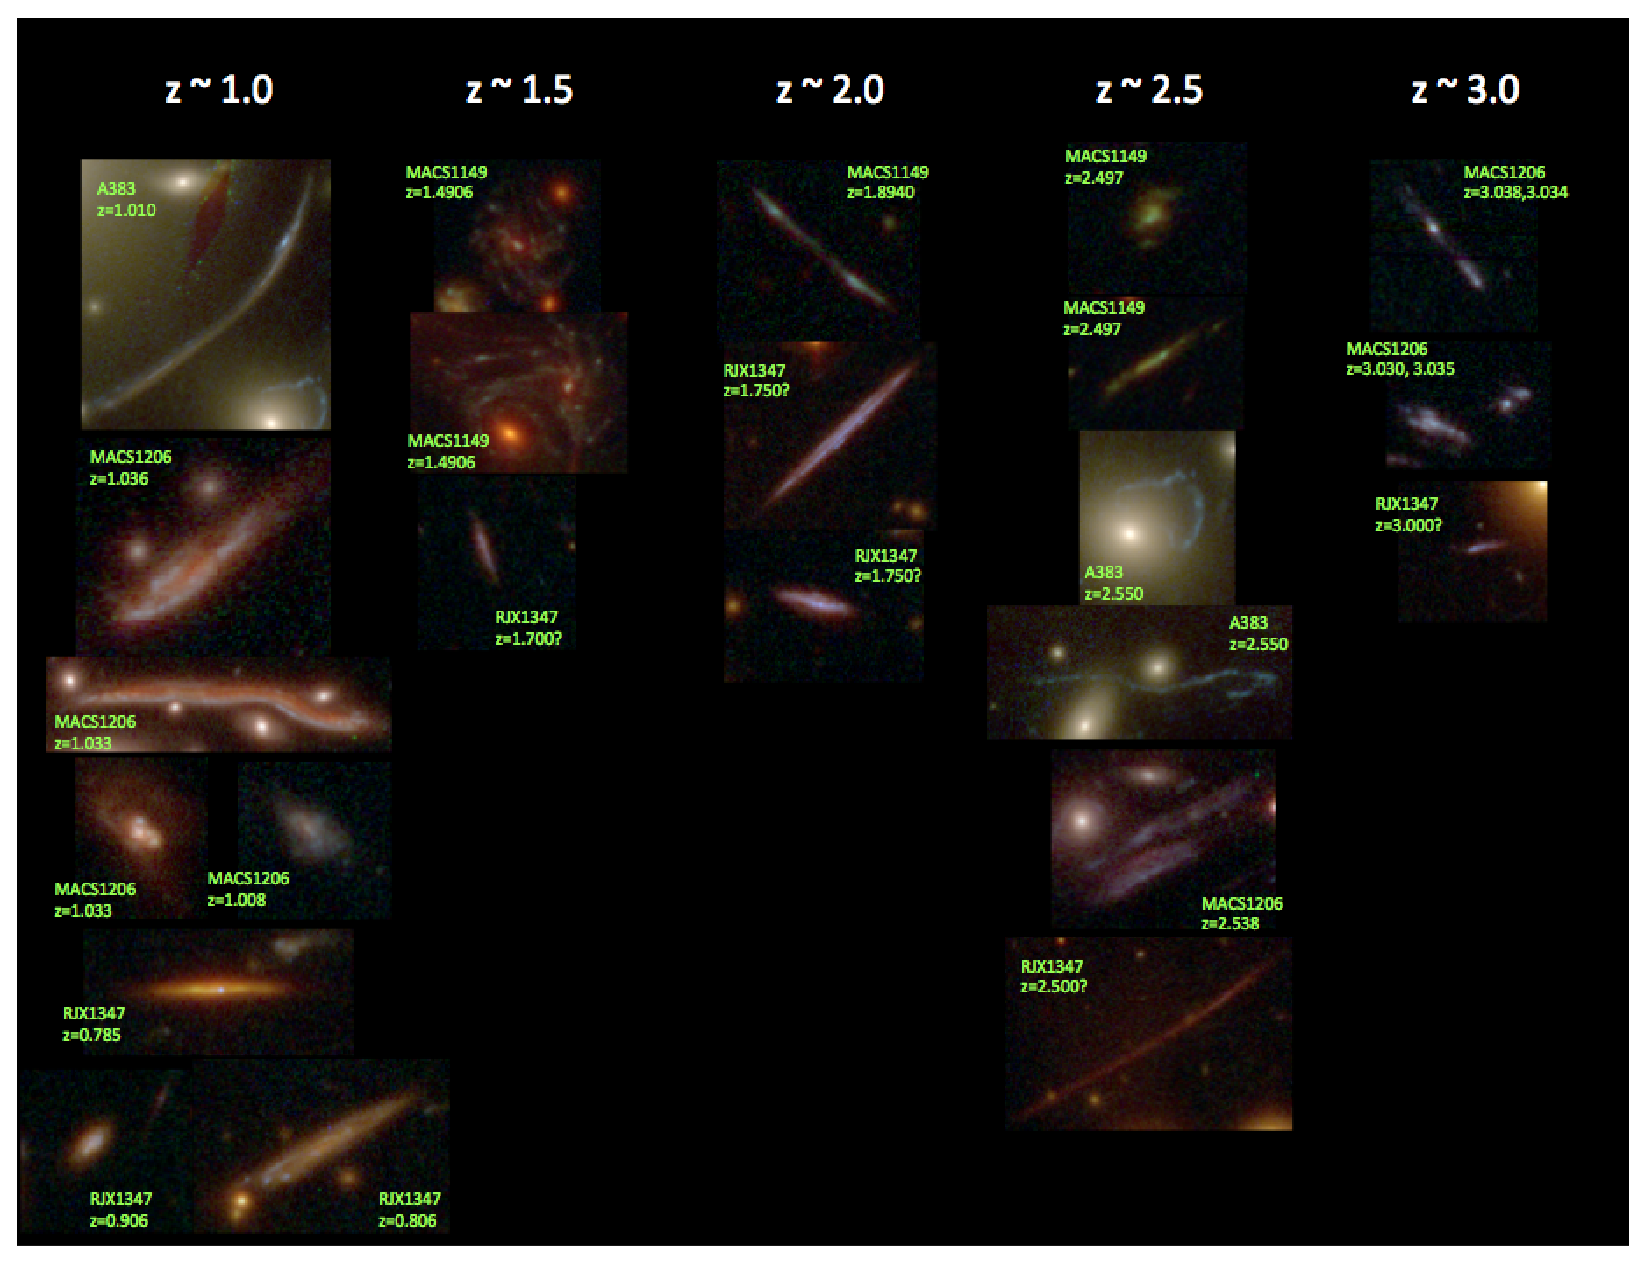
\includegraphics[width=1.0\linewidth]{candidates.eps}
\plotone{figures/candidates.eps}
\caption{Candidate targets for SED analysis, sorted by redshift.  For
  each candidate, the lensing cluster and redshift are indicated.
  More information about each candidate can be found in Table
  \ref{candidate_tab} including coordinates for locating each source.}
\label{candidate_fig}
\end{figure}


%%%%%%%%%%%%%%%%%%%%%%%% Imaging Data!! %%%%%%%%%%%%%%%%%%%

\section{Imaging Data}\label{imaging}

We will use the CLASH multi-band images that have been matched,
registered, and resampled to a common 30mas pixel grid.  Our SED
analysis measures the relative fluxes in different bands over matched
apertures; it is critical to have well-matched apertures in all
filters.  Apertures will be defined in the summed ``detection''
images, then applied in each individual filter.

The existing images have been resampled to a common scale, but have
different intrinsic resolution due to PSF variations.  To make a fair
comparison between the various filters without aperture problems, we
will convolve the higher resolution (compact PSF) images to match the
lowest resolution images in our filters.  {\bf{Open question:}} How do
we want to do the error analysis?  Do we need to make some kind of
error map and track the correlated errors generated by the PSF
convolution?

Background contamination from the BCG and other cluster members may be
a problem.  It might be best to do the final analysis on images in
which the BCG and other bright cluster members have been modeled and
subtracted.  Leonidas has suggested that Sara Ogaz's thumbnails of
individual galaxies and their GALFIT models might be useful here.  One
possibility is to add this to the InterCLASH interactive tool that he
and James Davies developed over the summer.  We may also want to make
use of Marc Postman's careful fits to the extended BCG light.

\vspace{0.08in}
\noindent{\bf{Ingredients:}}\vspace{-0.1in}
\begin{enumerate}\itemsep-6pt
\item The 16 individual drizzled images for each cluster containing a
  target.  {\bf{NOTE:}} 30mas images do not yet exist for all observed
  clusters! 
\item The weight map for each image.
\item The PSF (average over the field of view? as a function of
  location?) for each individual filter.
\item Sara's thumbnail images and GALFIT model fits to individual
  cluster members.
\item Marc's extended BCG fits for careful background subtraction.
\end{enumerate}

\noindent{\bf{Tasks:}}\vspace{-0.1in}
\begin{enumerate}\itemsep-6pt
\item Obtain the PSF for each filter.  
\item Convolve the images to a common effective resolution.
\item Construct error maps that treat the correlated errors from
  drizzling and PSF convolution in a reasonable way.
\item Implement a way to create images in which the BCG and other
  bright cluster members have been subtracted.  Create these images
  and use them (instead of? in addition to?) the raw images
  themselves.
\end{enumerate}


%%%%%%%%%%%%%%%%% A.U.S. (Apertures of Unusual Size) %%%%%%%%%%%%%%%%%

\section{Apertures of Unusual Size/Shape}\label{apertures}

Once the images have been resampled onto matching pixel grids and
convolved to have the same effective resolution, we can define
apertures of any size or shape by designating which pixels should be
included in each aperture.  This process involves deciding where to
draw the boundaries for each aperture, producing a list of pixels that
belong in each aperture, then computing the summed flux and
corresponding error values for each filter in each aperture.

Chien Peng has written tools that will be useful for this.  There are
two relevant programs.  The first, {\it{ds9poly.c}}, is a tool for
defining polygons interactively in DS9.  The second,
{\it{fillpoly.f}}, takes the polygon output from ds9poly and produces
a list of coordinates for all of the pixels that fall inside that
polygon.  A description of these tools can be found here on his ``Bad
Pixel Masking FAQ'' page. 

Once apertures have been defined and the pixels corresponding to each
aperture have been tabulated, we can sum the flux in the constituent
pixels for each aperture and compute errors on the summed aperture
fluxes.  {\bf{NOTE:}} We have to figure out how to deal with the
correlated errors in adjascent pixels due to drizzling and PSF
convolution.  

\vspace{0.08in}
\noindent{\bf{Ingredients:}}\vspace{-0.1in}
\begin{enumerate}\itemsep-6pt
\item {The routines {\it{ds9poly.c}} and {\it{fillpoly.f}} from Chien
  Peng's website.}
\item {Re-sampled, PSF convolved, (possibly BCG and cluster member
  subtracted) images for the cluster in each filter.}
\item {Error maps for each filter(?).}
\end{enumerate}

\noindent{\bf{Tasks:}}\vspace{-0.1in}
\begin{enumerate}\itemsep-6pt
\item {Download, install, and test {\it{ds9poly.c}} and
  {\it{fillpoly.f}}.}
\item {Choose apertures.}
\item {Run {\it{ds9poly}} and {\it{fillpoly}} to create pixel lists
  for each aperture.}
\item {Write an IDL code to take the 16 input *.fits images and
  aperture pixel lists and produce summed fluxes and errors in each
  band for each aperture.}
\end{enumerate}


%%%%%%%%%%%%%%%%% Stellar Population SED Fitting %%%%%%%%%%%%%%%%%

\section{Stellar Population SED Fitting}\label{SED_fit}

The first project goal is resolved SED fitting of stellar populations
in lensed galaxies.  This project may present the resolved fitting of
invidual objects on their own, or may aggregate the properties of many
objects to study resolved stellar populations at several different
redshifts.  

Once 16-band photometry has been computed in a given aperture, we will
use John's ISEDFIT code to fit the aperture SEDs.  Currently, John's
code is set up to run grids for several different stellar population
models: Bruzual-Charlot 2003, Maraston 2005, and Conroy's Flexible
Stellar Population Synthesis (FSPS).  Comparing results from the
various models will help constrain the systematics of using different
underlying models.  

There are several quantities of interest in the model results.  The
models will measure $M_{\star}$ values for the various galaxy
sub-components.  To interpret these masses, we will need to know the
magnification due to cluster lensing.  These values can be obtained
from the strong lensing analysis of the clusters.  Question: does the
magnification vary across the arcs?  Is this something we can hope to
constrain?  

ISEDFIT also produces best-fitting values of age, $Z$, star-formation
timescale $\tau$, and dust reddening $E(B-V)$.  It will be interesting
to compare the ages and star-formation timescales of different galaxy
components as measured in the various apertures.  One goal is to
constrain whether star formation in galaxies proceeds ``inside out''
or ``outside in''.  Tying the different apertures to actual locations
in the unlensed source will probably require deprojecting the lensed
galaxies back to the source plane.  This information can presumably be
obtained from the strong lensing analysis by other team members.

Another interesting aspect of the resolved stellar population analysis
will be to look for the presence of old stellar components,
particularly in high redshift galaxies.  The detection of truly
passive sub-components of high redshift galaxies might allow us to say
interesting things about bulge formation in galaxies.  

The stellar population information is sensitive to various
age/$Z$/dust degeneracies.  It will be important to track and quantify
these degeneracies, probably by looking at the full $\chi^2$
distribution in multi-dimensional parameter space.  In particular, I
think it will be interesting to explore the co-dependence of pairs of
parameters (e.g., age-$Z$, age-$\tau$, age-dust) while marginalizing
over other parameters.  

Depending on how bad the $Z$-related degeneracies are, it might be
possible to constrain the metallicities of different galaxy
sub-components.  Of particular interest would be to compare the $Z$
values of the most active star-forming regions with those of the older
stellar components to look for evidence of the source of the gas in
the star-forming knots.  Star formation that is triggered through
pristine gas accretion or merging with gas-rich low-mass (and
therefore low-$Z$) companions could produce low-$Z$ star-forming
regions, while ongoing quiescent star formation or major mergers (with
more equal mass and therefore more equal $Z$ companions) would
presumably result in higher-$Z$ star forming regions.  

\vspace{0.08in}
\noindent{\bf{Ingredients:}}\vspace{-0.1in}
\begin{enumerate}\itemsep-6pt
\item {The ISEDFIT code package, with reasonable pre-computed model
  grids.}
\item {The total aperture photometry from \S\ref{apertures}, along
  with errors.}
\item {Magnification maps and source plane reconstructed morphologies
  for the lensed galaxies from the strong lensing analysis by other
  team members.}
\end{enumerate}

\noindent{\bf{Tasks:}}\vspace{-0.1in}
\begin{enumerate}\itemsep-6pt
\item {Decide which model grids to use for ISEDFIT.  If we want
  anything other than the 3 pre-computed models for ISEDFIT, we will
  need to produce them.}
\item {Run ISEDFIT on the aperture photometry from \S\ref{apertures}.}
\item {Explore the $\chi^2$ distribution in the multi-dimensional
  input parameter space in order to constrain the various stellar
  population modelling degeneracies.}
\item {Do science!!!}
\end{enumerate}


% %%%%%%%%%%%%%%%%% Dust SED Fitting %%%%%%%%%%%%%%%%%
% 
% \section{Fitting the Dust SED}\label{dust_fit}
% 
% Some of the strongly-lensed background galaxies appear to be edge-on
% star forming galaxies with strong, patchy dust obscuration.  The
% 16-band HST photometry of these resolved, extended objects makes this
% data set an ideal place to characterize the dust absorption SED in
% various targets and at various redshifts.  This second project will
% define obscured and un-obscured apertures within individual lensed
% galaxies and, by assuming that the intrinsic SED of the dust-obscured
% material is the same as that of the unobscured material, use the
% difference between the obscured and un-obscured SEDs to measure the
% SED of the dust absorption.  
% 
% This is an entirely empirical comparison and therefore does not (in
% its simplest version) involve the use of ISEDFIT.  However, it might
% be very interesting to measure the dust SED as a function of host
% galaxy mass (and therefore presumably host galaxy $Z$), which would
% require $M_{\star}$ estimates from ISEDFIT.  Dealing with the heavily
% dust-obscured apertures in ISEDFIT might be complicated---we'd have to
% figure out how we would do that.
% 
% 
% \vspace{0.08in}
% \noindent{\bf{Ingredients:}}\vspace{-0.1in}
% \begin{enumerate}\itemsep-6pt
% \item {The total aperture photometry from \S\ref{apertures}, along
%   with errors.}
% \item {Magnification maps and source plane reconstructed morphologies
%   for the lensed galaxies from the strong lensing analysis by other
%   team members (only necessary if making $M_{\star}$ estimates).}
% \item {The ISEDFIT code package, with reasonable pre-computed model
%   grids (only necessary if making $M_{\star}$ estimates).}
% \end{enumerate}
% 
% \noindent{\bf{Tasks:}}\vspace{-0.1in}
% \begin{enumerate}\itemsep-6pt
% \item {Construct the obscured and un-obscured galaxy SEDs.  Compare
%   them.}
% \item {Do science!!!}
% \end{enumerate}



\acknowledgements

The work of LAM was carried out at Jet Propulsion Laboratory, California
Institute of Technology, under a contract with NASA. 

\bibliographystyle{apj}
\bibliography{/Users/leonidas/Dropbox/bibdesk/moustakasbibs.bib}

\end{document}
